\chapter{Metodologia e strumenti utilizzati}
Nel capitolo dedicato alla metodologia e agli strumenti utilizzati, vengono delineati i principi fondamentali che guidano la ricerca, nonché le tecniche e le tecnologie impiegate per raggiungere gli obiettivi prefissati. Questo capitolo fornisce una panoramica delle scelte metodologiche adottate, con particolare attenzione all'approccio di Data Augmentation e all'impiego di dati simulati per ottimizzare l'addestramento dei sistemi di rilevamento delle intrusioni (IDS). Verranno descritti i modelli e gli algoritmi di machine learning selezionati, oltre agli strumenti software utilizzati per l'analisi dei dati e la valutazione delle prestazioni dei modelli. Questa sezione è fondamentale per comprendere il contesto in cui si inserisce la ricerca e per garantire la riproducibilità dei risultati ottenuti.

\section{Workflow}

In questa sezione, verranno chiariti l'obiettivo della tesi e il flusso di lavoro seguito per raggiungerlo. L'obiettivo principale è valutare come variano le performance dell'IDS adottando un approccio di Data Augmentation. In particolare, si vuole esaminare l'impatto di questa tecnica nel migliorare la capacità del sistema di rilevare anomalie e attacchi in contesti IoT. Il workflow descritto in figura fornisce una panoramica dettagliata delle fasi seguite durante l'intero processo. Di seguito, descriviamo le varie fasi operative:

\begin{figure}[htbp]
\centering
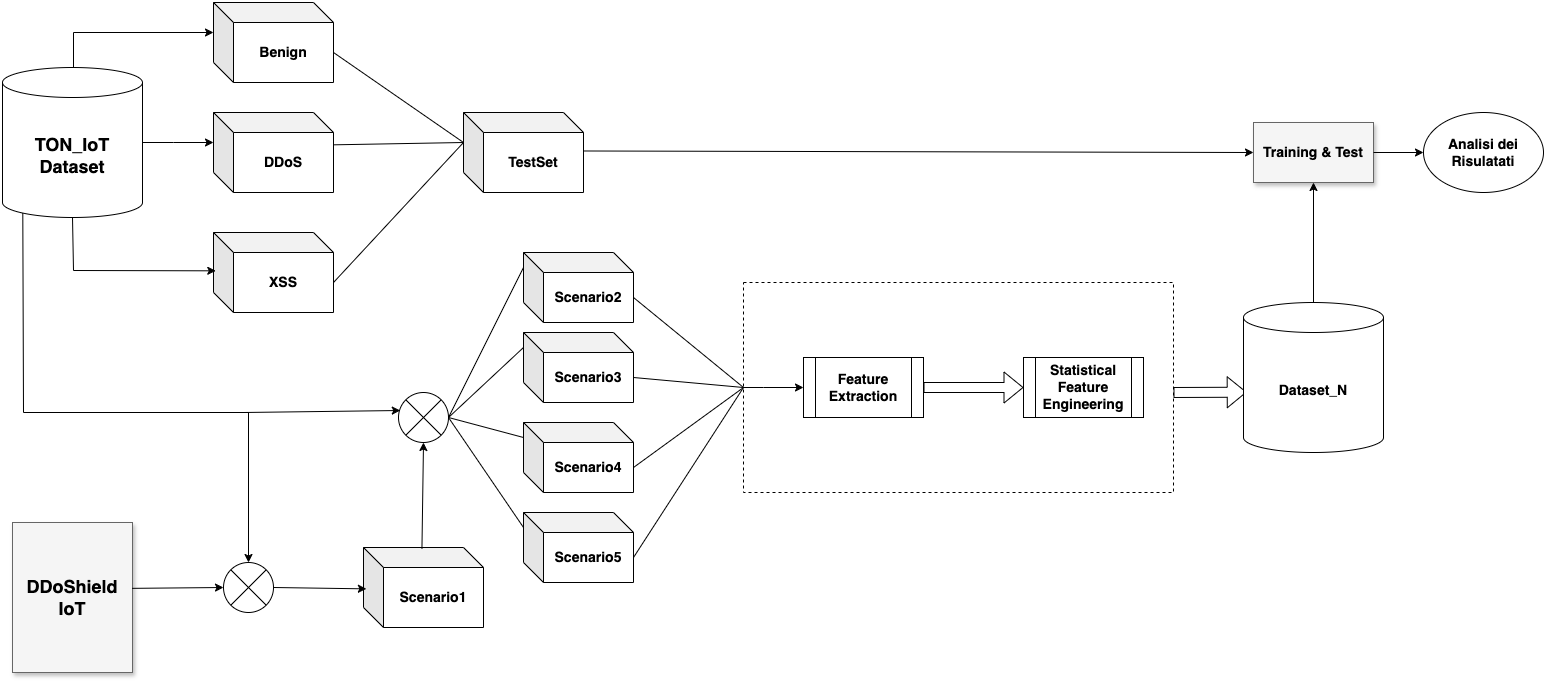
\includegraphics[scale= 0.27]{UNINA_MSc_Thesis_Project/img/chapterMetodologia/Workflow_Bold_XXL.png}
  \caption{Workflow seguito}
\end{figure}


\begin{itemize}
    \item \textbf{Definizione e creazione di diversi scenari}: Per rappresentare una varietà di situazioni e contesti di rete, sono stati creati più scenari che simulano condizioni reali, inclusi diversi tipi di traffico di rete e differenti intensità di attacco DDoS. Questi scenari permettono di valutare le prestazioni dell'IDS in ambienti eterogenei.
    
    \item \textbf{Raccolta dei dati}: I dati sono stati acquisiti attraverso il tool \texttt{tcpdump}, che fa parte della suite Wireshark. Questo strumento ha permesso di catturare il traffico di rete sia benigno che malevolo, generando un dataset realistico per l'addestramento e la valutazione dei modelli di rilevamento delle intrusioni.
    
    \item \textbf{Estrazione delle feature di interesse}: Dopo la raccolta dei dati, è stato effettuato un processo di estrazione delle feature che ci interessano maggiormente per il rilevamento delle anomalie. Queste feature includono parametri relativi al traffico, come la dimensione dei pacchetti, il tempo di trasmissione e il numero di pacchetti inviati in una finestra temporale definita.
    
    \item \textbf{Processo di feature engineering}: Successivamente, si è proceduto con un processo di feature engineering per migliorare la qualità dei dati e ottimizzare le feature utilizzate per l'addestramento. Questo passaggio è fondamentale per aumentare l'efficacia del modello e ridurre l'overfitting, migliorando così la sua capacità di generalizzare su nuovi dati.
    
    \item \textbf{Creazione di un test set}: È stato creato un test set separato, composto da dati non utilizzati nella fase di addestramento, per valutare in maniera imparziale le performance dei modelli di rilevamento. Il test set include sia traffico benigno che attacchi simulati, con lo scopo di testare la capacità dell'IDS di distinguere tra i due.
    
    \item \textbf{Analisi e discussione dei risultati}: Una volta addestrati e testati i modelli, è stata eseguita un'analisi approfondita dei risultati. Questa fase include la valutazione delle metriche di performance (come accuratezza, precisione, recall e F1-score), e la discussione sull'impatto della Data Augmentation sulle prestazioni dell'IDS, mettendo in evidenza i vantaggi e le limitazioni della tecnica adottata.
\end{itemize}

Il workflow descritto assicura una metodologia rigorosa e riproducibile per valutare l'efficacia dell'uso della Data Augmentation nel migliorare le performance degli IDS in ambienti IoT. Ogni fase è stata eseguita con l'obiettivo di massimizzare la generalizzazione del modello e di ottenere un quadro dettagliato delle sue capacità in scenari complessi e variabili.

\section{Scenari Riprodotti}
I dataset utilizzati in questo lavoro sono stati costruiti con l'obiettivo di fornire una varietà di scenari di traffico di rete, con diverse distribuzioni di attacchi e protocolli, al fine di testare e addestrare modelli di rilevamento delle intrusioni. I dataset sono suddivisi in cinque diverse configurazioni, ciascuna caratterizzata da una combinazione specifica di traffico benigno e maligno, con l'aggiunta o la rimozione del contributo di un simulatore che verrà introdotto in seguito. Questa diversificazione consente di analizzare l'efficacia degli \textit{IDS} su scenari realistici e variabili, riflettendo le condizioni tipiche delle reti IoT.

\textbf{Dataset 1}: Il primo dataset rappresenta la base su cui sono stati costruiti tutti gli altri. Esso è costituito da una porzione del traffico benigno del \textit{TON\_IoT dataset} combinato con il traffico generato dal simulatore \textit{DDoShield}, che include sia traffico benigno che maligno. Questo dataset contiene un totale di circa 1.670.000 pacchetti, con una distribuzione di circa 57.34\% di pacchetti benigni e 42.66\% di pacchetti maligni appartenenti ad attacchi DDoS. A partire da questo dataset, frazionando il traffico maligno saranno generati gli altri scenari.

\begin{figure}[htbp]
\centering
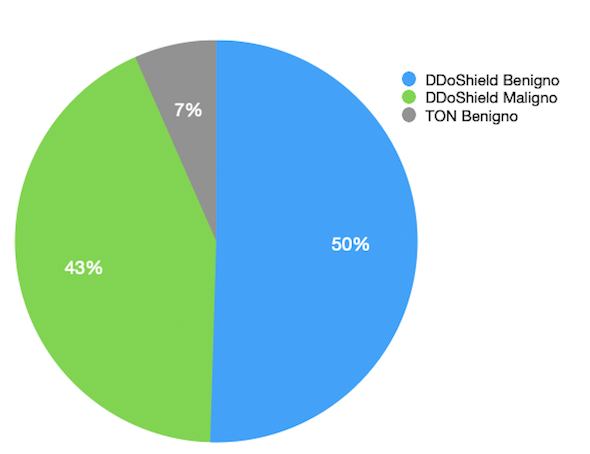
\includegraphics[scale= 0.8]{UNINA_MSc_Thesis_Project/img/chapterRisulati/composizione_DATASET_1 centrata.png}
  \caption{Composizione Dataset 1}
\end{figure}

\textbf{Dataset 2}: Questo dataset è stato creato mantenendo invariato il traffico benigno del \textit{Dataset 1} e frazionando il traffico maligno del \textit{DDoShield}. La suddivisione del traffico maligno è stata fatta in modo equo, con il 50\% di pacchetti provenienti dal \textit{DDoShield} e il 50\% provenienti dal \textit{TON\_IoT}, limitati all'attacco \textit{DDoS}. Questo dataset è particolarmente utile per testare la capacità degli \textit{IDS} di rilevare attacchi \textit{DDoS} distribuiti su diverse fonti.

\begin{figure}[htbp]
\centering
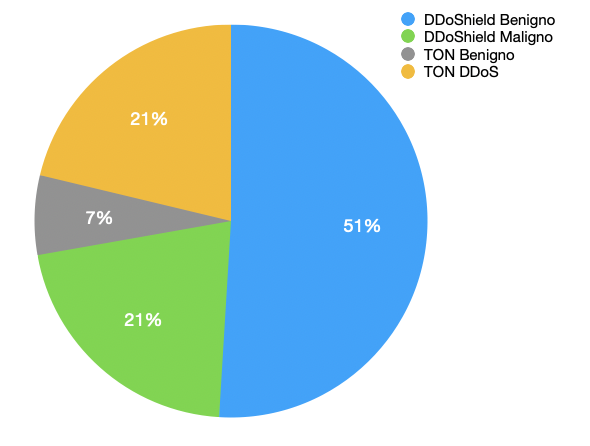
\includegraphics[scale= 0.8]{UNINA_MSc_Thesis_Project/img/chapterRisulati/composizione_DATASET_2.png}
  \caption{Composizione Dataset 2}
\end{figure}

\textbf{Dataset 3}: Il terzo dataset segue una logica simile al \textit{Dataset 2}, ma con una diversa distribuzione del traffico maligno: il 70\% del traffico maligno proviene dal \textit{DDoShield}, mentre il restante 30\% dal \textit{TON\_IoT} con attacchi \textit{DDoS}. Questa configurazione aumenta l'enfasi sugli attacchi simulati rispetto a quelli reali, creando uno scenario più complesso in cui testare la capacità di generalizzazione degli \textit{IDS} di fronte a differenti fonti di attacco.

\begin{figure}[htbp]
\centering
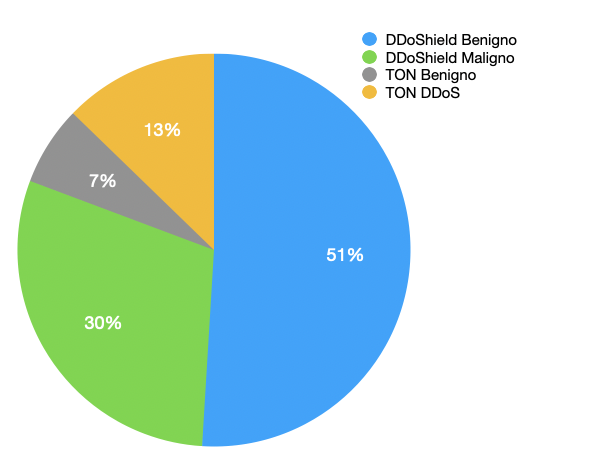
\includegraphics[scale= 0.8]{UNINA_MSc_Thesis_Project/img/chapterRisulati/composizione_DATASET_3.png}
  \caption{Composizione Dataset 3}
\end{figure}

\textbf{Dataset 4}: Questo dataset inverte la proporzione del traffico maligno rispetto al \textit{Dataset 3}, con il 30\% proveniente dal \textit{DDoShield} e il 70\% dal \textit{TON\_IoT} (sempre con attacchi \textit{DDoS}). Questa configurazione è particolarmente importante per testare la robustezza degli \textit{IDS} nei confronti di attacchi reali con una bassa interferenza di dati simulati. La prevalenza di traffico \textit{DDoS} reale rende questo dataset utile per l'analisi della capacità del sistema di rilevare minacce realistiche in ambienti IoT.

\begin{figure}[htbp]
\centering
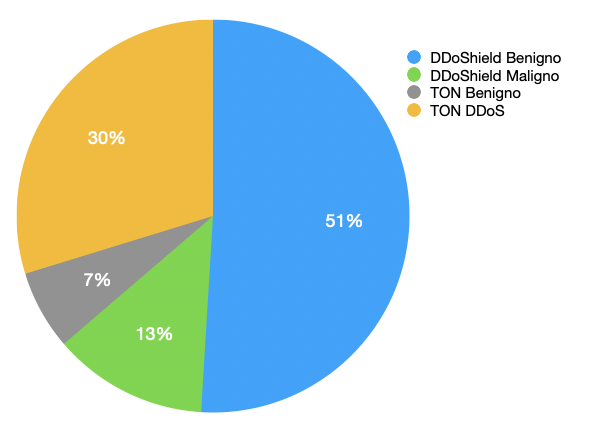
\includegraphics[scale= 0.8]{UNINA_MSc_Thesis_Project/img/chapterRisulati/composizione_DATASET_4.png}
  \caption{Composizione Dataset 4}
\end{figure}

\textbf{Dataset 5}: Questo dataset introduce una maggiore complessità includendo non solo attacchi \textit{DDoS}, ma anche attacchi \textit{XSS} (\textit{Cross-Site Scripting}) provenienti dal \textit{TON\_IoT dataset}. In questa configurazione, il traffico maligno è suddiviso equamente tra il 50\% di pacchetti provenienti dal \textit{DDoShield} e il 50\% proveniente dal \textit{TON\_IoT}, ulteriormente frazionato in 25\% \textit{DDoS} e 25\% \textit{XSS}. Questo dataset rappresenta uno scenario multi-attacco complesso, che mette alla prova la capacità degli \textit{IDS} di gestire simultaneamente più tipologie di minacce, rendendo particolarmente interessante l'analisi della loro capacità di distinguere fra attacchi di natura diversa.

\begin{figure}[htbp]
\centering
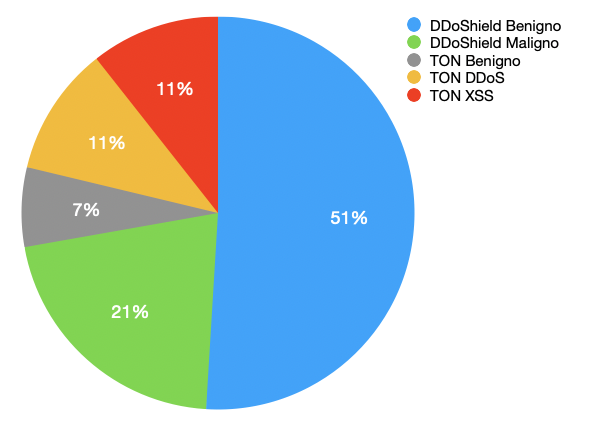
\includegraphics[scale= 0.8]{UNINA_MSc_Thesis_Project/img/chapterRisulati/composizione_DATASET_5.png}
  \caption{Composizione Dataset 5}
\end{figure}

La scelta delle percentuali è finalizzata a riprodurre condizioni diverse e quindi scenari favorevoli e sfavoreli con lo scopo ultimo di isolare l'impatto del simulatore e trovare il giusto compromesso per l'addestramento degli IDS.

Per valutare gli scenari descritti, è stato creato un \textit{test set} della dimensione pari al 20\% dei \textit{dataset}, ottenuto tramite un campionamento casuale di pacchetti non presenti nel set di \textit{train} estratti dal \textit{TON\_IoT dataset}. La scelta di utilizzare il 20\% deriva dalla necessità di avere una porzione di dati sufficientemente rappresentativa per testare il modello, senza però compromettere la quantità di dati disponibili per l'addestramento. Questo rapporto tra \textit{train} e \textit{test} è comunemente adottato in ambito di machine learning per garantire che il modello sia esposto a una varietà adeguata di pattern durante la fase di addestramento, mantenendo al contempo una solida base di dati indipendenti per la valutazione delle prestazioni.

Inoltre, la selezione casuale garantisce che il \textit{test set} contenga una distribuzione rappresentativa sia di traffico benigno che di traffico maligno, minimizzando così il rischio di bias e garantendo una valutazione più robusta del modello. Con un \textit{test set} ben bilanciato e di dimensioni adeguate, è possibile ottenere una stima più accurata della generalizzazione del modello a nuovi dati non visti, condizione essenziale per il deployment in scenari reali, come la protezione di reti IoT. \cite{DeepLearning}

\section{Tecniche di rilevamento delle anomalie}
Negli IDS basati su un approccio \textit{anomaly-based}, come abbiamo visto nel capitolo precedente, la vasta quantità di dati da analizzare può rendere complesso individuare anomalie in tempo reale. Di conseguenza, la scelta della tecnica utilizzata per il rilevamento assume un'importanza cruciale. Nei paragrafi seguenti, forniremo una panoramica di queste tecniche, evidenziando i vantaggi e le limitazioni di ciascuna.
%TODO: Forse questo pezzettino è da aggiustare o comunque riformulare il concetto, ASPETTA di avere più chiaro l'ordine del capitolo 
Abbiamo già discusso le principali differenze tra un approccio basato su firme e uno basato sul rilevamento delle anomalie. Ora possiamo approfondire le possibili soluzioni implementative per quest'ultimo approccio, che mira a individuare comportamenti anomali rispetto al normale funzionamento del sistema. Questi metodi, pur avendo vantaggi significativi, richiedono una gestione attenta del modello e dei dati, poiché un numero elevato di falsi positivi potrebbe rendere il sistema meno efficace. Esploriamo di seguito alcune delle principali tecniche adottate nell'ambito del rilevamento delle anomalie:

\begin{longtable}{|p{3cm}|p{3cm}|p{4cm}|p{4cm}|}
\hline
\textbf{Tecniche} & \textbf{Modelli} & \textbf{Vantaggi} & \textbf{Svantaggi} \\
\hline
\endfirsthead % Intestazione della prima pagina
\hline
\textbf{Tecniche} & \textbf{Modelli} & \textbf{Vantaggi} & \textbf{Svantaggi} \\
\hline
\endhead % Intestazione delle pagine successive

\multirow{4}{3cm}{\raggedright \textbf{Basato su firme}} 
 & • Confronto di pattern & • Alta accuratezza per attacchi noti & • Incapacità di rilevare attacchi nuovi o sconosciuti \\
 & • Analisi dei protocolli & • Basso tasso di falsi positivi & • Dipendenza dagli aggiornamenti delle firme \\
 & • Ispezione dei contenuti & • Facile da implementare & • Mancanza di flessibilità \\
 & • Analisi dei log & • Basso overhead computazionale & • Copertura limitata \\
\hline
\multirow{3}{3cm}{\raggedright \textbf{Modelli Statistici}} 
 & • Rilevamento di anomalie & • Metodo consolidato con una solida base teorica & • Capacità limitata di rilevare anomalie complesse o sofisticate \\
 & • Analisi delle serie temporali & • Adatto per il rilevamento di anomalie semplici & • Sensibilità alla distribuzione dei dati e alle assunzioni \\
 & • Modellazione statistica & • Risultati interpretabili & • Difficoltà nella gestione di dati ad alta dimensionalità \\
\hline
\multirow{4}{3cm}{\raggedright \textbf{Machine Learning}} 
 & • Clustering & • Capacità di gestire pattern complessi e non lineari & • Necessità di grandi set di dati etichettati per l'addestramento \\
 & • Classificazione & • Efficace per identificare anomalie sottili & • Possibile overfitting se non ottimizzato correttamente \\
 & • Reti neurali & • Adattabilità a ambienti mutevoli & • Complessità computazionale elevata per algoritmi complessi \\
 &  & • Può apprendere da dati non etichettati o parzialmente etichettati & • La natura "black-box" può limitare l'interpretabilità \\
\hline
\multirow{4}{3cm}{\raggedright \textbf{Approcci Ibridi}} 
 & • Modelli Statistici + Machine Learning & • Sfruttare i punti forti di entrambe le tecniche & • Aumenta la complessità del sistema e della sua integrazione \\
 &  & • Precisione ed affidabilità migliorate & • Risorse computazionali più elevate \\
 &  & • Maggiori capacità di gestire diverse anomalie &  \\
\hline
\caption{Confronto tra tecniche IDS, modelli, vantaggi e svantaggi}
\label{tab:confronto_ids}
\end{longtable}

\begin{itemize}
\item \textbf{Approccio statistico}: Questo metodo si basa su modelli matematici che analizzano il comportamento storico del sistema per stabilire una baseline, o comportamento normale. Le deviazioni significative da questa baseline vengono interpretate come potenziali anomalie. Gli approcci statistici possono includere tecniche come il calcolo della media, deviazione standard, analisi della varianza e regressione. Sebbene siano semplici da implementare, possono risultare inefficaci in ambienti dinamici dove il comportamento normale cambia frequentemente, portando a falsi positivi o falsi negativi.

\item \textbf{Approccio con tecniche di Machine Learning}: L'utilizzo di algoritmi di apprendimento automatico rappresenta una soluzione avanzata per il rilevamento delle anomalie. Attraverso l'addestramento su grandi quantità di dati storici, un modello di machine learning può apprendere a distinguere tra comportamenti normali e anomali. Gli algoritmi di apprendimento possono seguire due tipi di approccio: quello \textbf{supervisionato}, che include tecniche come le reti neurali o gli alberi decisionali, e richiede un dataset etichettato per l'addestramento; e quello \textbf{non supervisionato}, che comprende metodi come il clustering o gli autoencoder, i quali non necessitano di etichette e possono identificare anomalie senza una conoscenza preliminare.

Il primo approccio è particolarmente efficace per il rilevamento di anomalie già note, ma presenta limitazioni quando si tratta di individuare nuove anomalie. Al contrario, il secondo approccio offre maggiore flessibilità, ma la sua efficacia è strettamente legata alla qualità e alla quantità dei dati utilizzati per l'addestramento. In molti contesti applicativi, non c'è disponibilità di dati pre-etichettati, motivo per cui gli algoritmi di machine learning non supervisionati sono spesso preferiti.

\begin{figure}[htbp]
\centering
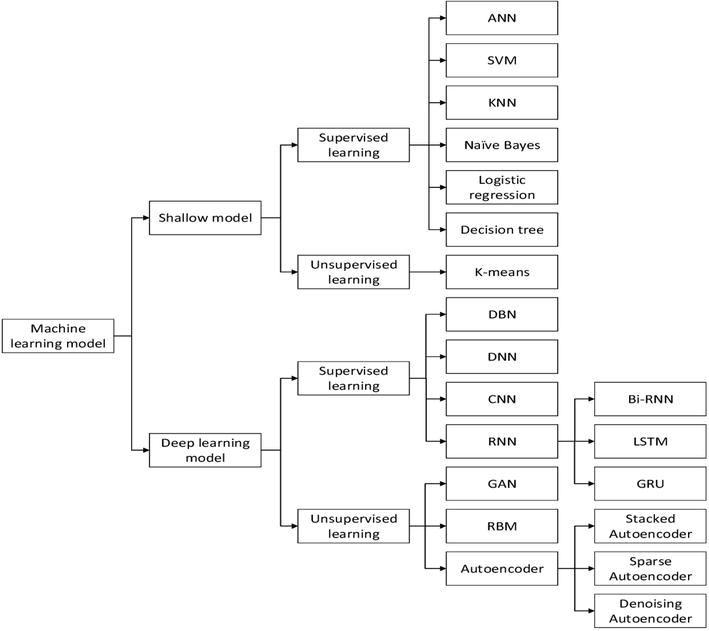
\includegraphics[scale= 0.9]{UNINA_MSc_Thesis_Project/img/chapterMetodologia/machineLearnin_models.png}
  \caption{Famiglie di Modelli di Machine Learning}
\end{figure}

\item \textbf{Approcci ibridi}: Gli approcci ibridi combinano tecniche statistiche e di machine learning per migliorare l'accuratezza e l'efficacia del rilevamento delle anomalie negli IDS. Sfruttando i punti di forza di entrambe le metodologie, i modelli ibridi offrono capacità di rilevamento più avanzate e complete. Ad esempio, un approccio ibrido può utilizzare tecniche statistiche per definire il comportamento di base del sistema e algoritmi di machine learning per classificare le istanze come normali o anomale. Questa combinazione permette di realizzare un sistema di rilevamento delle anomalie più completo e robusto. \cite{AnomalyDetection}
\end{itemize}

\section{Algoritmi Utilizzati per l'Addestramento}

In questa sezione vengono descritti gli algoritmi utilizzati per l'addestramento dei modelli di IDS: \textit{K-Means}, \textit{Random Forest (RF)} e \textit{Convolutional Neural Network (CNN)}. Questi algoritmi sono stati scelti per le loro capacità di gestire grandi quantità di dati e rilevare pattern complessi in contesti di sicurezza informatica.

\subsection{K-Means}

\textit{K-Means} è un algoritmo di clustering non supervisionato utilizzato per suddividere un insieme di dati in $k$ gruppi, dove ogni gruppo è rappresentato dal suo centroide. L'algoritmo funziona iterativamente per minimizzare la varianza interna ai cluster, cercando di assegnare ciascun punto dati al cluster con il centroide più vicino. L'obiettivo è trovare una suddivisione che minimizzi la distanza quadratica totale tra i punti e i loro centroidi.

\[
J = \sum_{i=1}^{k} \sum_{x \in C_i} \left\| x - \mu_i \right\|^2
\]

Dove:
\begin{itemize}
    \item $C_i$ rappresenta il $i$-esimo cluster.
    \item $\mu_i$ è il centroide del $i$-esimo cluster.
\end{itemize}

K-Means è stato utilizzato in questo lavoro per effettuare un raggruppamento dei dati, in modo da identificare potenziali gruppi di traffico maligno e benigno senza etichette supervisionate.
\cite{K_Means}

\subsection{Random Forest (RF)}

\textit{Random Forest} è un algoritmo di apprendimento supervisionato basato su alberi decisionali. Il modello costruisce una "foresta" di alberi decisionali, ognuno addestrato su un sottoinsieme casuale dei dati. La previsione finale viene ottenuta facendo la media delle previsioni di tutti gli alberi (per problemi di regressione) o votando la classe più frequente (per problemi di classificazione).

L'algoritmo Random Forest è particolarmente efficace per i dataset con molti attributi e per problemi complessi in cui sono presenti interazioni non lineari tra le variabili. In questo contesto, è stato utilizzato per classificare il traffico di rete come benigno o maligno, fornendo buone prestazioni in termini di precisione e capacità di gestione di grandi volumi di dati. \cite{RandomForest}

\subsection{Convolutional Neural Network (CNN)}

Le \textit{Convolutional Neural Networks (CNN)} sono una classe di reti neurali profonde particolarmente efficaci nell'elaborazione di dati strutturati come immagini o sequenze temporali. Nel contesto di questo lavoro, le CNN sono state utilizzate per classificare il traffico di rete, trattando i pacchetti di dati come una sorta di immagine temporale, permettendo alla rete di catturare pattern locali e rilevare anomalie nel traffico.

Le CNN si basano su strati convolutivi che applicano filtri convoluzionali ai dati in input, seguiti da strati di pooling che riducono la dimensionalità. Infine, uno o più strati completamente connessi (fully connected) combinano le informazioni estratte dai layer precedenti per effettuare la classificazione finale.

\[
y = f(\mathbf{W} * \mathbf{x} + \mathbf{b})
\]

Dove:
\begin{itemize}
    \item $\mathbf{x}$ è l'input (ad esempio, un segmento del traffico di rete).
    \item $\mathbf{W}$ sono i filtri convoluzionali applicati.
    \item $\mathbf{b}$ è il bias.
    \item $f$ è una funzione di attivazione non lineare, tipicamente ReLU.
\end{itemize}

Le CNN si sono dimostrate efficaci nell'individuare pattern complessi e ripetitivi nel traffico di rete, migliorando la capacità di rilevamento di attacchi sofisticati come DDoS e XSS.\cite{CNN}

\section{Metriche utilizzate}

Per la valutazione delle prestazioni dei modelli di rilevamento delle intrusioni (\textit{Intrusion Detection Systems}, IDS) addestrati sui vari dataset descritti in precedenza, sono state utilizzate le seguenti metriche: \textbf{Accuracy}, \textbf{Precision}, \textbf{Recall} e \textbf{F1-score}. Queste metriche sono ampiamente utilizzate in ambito di machine learning per valutare la capacità dei modelli di classificazione binaria (traffico benigno e traffico maligno) di distinguere correttamente tra classi positive (attacchi) e negative (traffico legittimo).
Prima di procedere con la discussione delle metriche, definiamo alcune espressioni utilizzate per le definzioni :
\begin{itemize}
    \item \textit{TP} (True Positives) sono i casi di attacchi rilevati correttamente.
    \item \textit{TN} (True Negatives) sono i casi di traffico benigno classificati correttamente.
    \item \textit{FP} (False Positives) sono i casi di traffico benigno classificati erroneamente come attacchi.
    \item \textit{FN} (False Negatives) sono i casi di attacchi non rilevati, classificati come traffico benigno.
\end{itemize}

\subsection{Accuracy}

L'\textbf{accuracy} (o accuratezza) misura la proporzione di predizioni corrette rispetto al totale delle predizioni effettuate. Tuttavia, in contesti come la rilevazione di intrusioni, dove i dati possono essere sbilanciati (con più traffico benigno rispetto a quello maligno), l'accuracy può non essere una metrica rappresentativa. Ad esempio, un modello che classifica tutto come benigno può comunque ottenere un'alta accuracy se la maggior parte dei dati appartiene alla classe benigna.

La formula per l'accuracy è la seguente:

\[
\text{Accuracy} = \frac{\textit{correct classifications}}{\textit{total classifications}}= \frac{TP + TN}{TP + TN + FP + FN}
\]

\subsection{Precision}

La \textbf{precision} (o precisione) indica la proporzione di predizioni positive corrette rispetto al totale delle predizioni positive effettuate. È particolarmente importante in contesti dove il costo di un falso allarme (FP) è elevato, come negli IDS, dove classificare erroneamente il traffico benigno come maligno potrebbe portare a un dispendio di risorse per l'analisi e la mitigazione di attacchi inesistenti.

La formula per la precision è:

\[
\text{Precision} =\frac{\textit{correctly classified actual postives}}{\textit{everything classified as positive}} = \frac{TP}{TP + FP}
\]

Una precisione elevata implica che il modello tende a essere conservativo nel dichiarare un attacco, riducendo così il numero di falsi positivi.

\subsection{Recall}

Il \textbf{recall} (o richiamo, talvolta anche noto come sensibilità o recupero) misura la proporzione di attacchi rilevati correttamente rispetto al totale degli attacchi presenti nel dataset. È una metrica critica in ambienti di sicurezza informatica, dove la mancata rilevazione di un attacco (FN) può avere conseguenze disastrose.

La formula per il recall è:

\[
\text{Recall} = \frac{\textit{correctly classified actual positves}}{\textit{all actual positives}}  = \frac{TP}{TP + FN}
\]

Un alto recall indica che il modello è in grado di rilevare la maggior parte degli attacchi, ma potrebbe essere a discapito di una maggiore presenza di falsi positivi.

\subsection{F1-score}

L'\textbf{F1-score} è la media armonica tra precision e recall e rappresenta un compromesso tra le due metriche. È particolarmente utile quando c'è uno squilibrio tra le classi, come nel caso degli attacchi rispetto al traffico legittimo in reti IoT, e quando si vuole bilanciare l'importanza del richiamo e della precisione.

La formula per l'F1-score è:

\[
\text{F1-score} = 2 \times \frac{\text{Precision} \times \text{Recall}}{\text{Precision} + \text{Recall}}
\]

Un F1-score elevato indica che il modello mantiene un buon equilibrio tra precisione e richiamo, riducendo sia i falsi positivi che i falsi negativi. \cite{metricsReference}

\subsection{Impatto delle metriche}

Nel contesto di questo lavoro di tesi, le metriche appena introdotte sono fondamentali per valutare l'efficacia delle tecniche di Data Augmentation applicate ai modelli di IDS. In particolare:
\begin{itemize}
    \item \textbf{Accuracy}: Sebbene utile come metrica generale, la sua interpretazione va fatta con cautela, specialmente nel caso di dataset sbilanciati, dove la percentuale di traffico benigno supera di gran lunga quella degli attacchi.
    \item \textbf{Precision}: È critica per ridurre i falsi positivi in scenari reali, dove classificare erroneamente il traffico benigno come maligno può generare falsi allarmi, aumentando i costi operativi.
    \item \textbf{Recall}: È di vitale importanza per garantire che il sistema di rilevamento catturi la maggior parte degli attacchi. Un recall basso può comportare il mancato rilevamento di attacchi critici, compromettendo la sicurezza delle reti IoT.
    \item \textbf{F1-score}: Permette di trovare un equilibrio ottimale tra precision e recall, rendendolo un indicatore chiave per valutare la robustezza dei modelli di IDS in scenari multi-attacco come quelli simulati nei dataset generati.
\end{itemize}

La valutazione dei modelli attraverso queste metriche consente di misurare non solo l'accuratezza complessiva, ma anche la capacità di generalizzazione dei modelli a nuovi dati non visti, garantendo che l'IDS possa essere implementato efficacemente in scenari reali con minacce dinamiche e varie.
